\documentclass[12pt]{article}

\usepackage{algorithm}
\usepackage{algpseudocode}
\usepackage{amsmath}
\usepackage{fullpage}
\usepackage{graphicx}
\usepackage{color}
\date{}
%\thispagestyle{empty}

\begin{document}

\begin{center}
	\fbox{
		\begin{tabular}{l}
			
\includegraphics[scale=0.75]{logo.png}
		\end{tabular} \hspace{0.5cm}
		\begin{tabular}{c}
			\color{red}{Indian Institute of Information Technology} \\
			\color{red}{Design and Manufacturing, Kancheepuram} \\
			Chennai – 600 127,  India \\
			\color{blue}{\small An Autonomous Institute under MHRD, Govt of India} \\
			\color{blue}{http://www.iiitdm.ac.in} \\ \hspace{0.2cm}
			COM306T-Automata and Compiler Design
		\end{tabular}
		\begin{tabular}{c}
			\color{blue}{Instructor} \\
			Dr. V. Masilamani \\
			Scribe: Vignesh Sairaj\\ 
		\end{tabular}
	}
\end{center}

\begin{center}
	Lecture-36 {\tt Syntax tree construction from annotated parse tree using post order traversal, and also during parsing(using SDD)}
\end{center}

\section{Introduction}
	\subsection{Parse Tree (Concrete Syntax Tree)}
	Given a CFG, a Parse tree is any ordered tree that satisfies the following properties:
	\begin{itemize}
		\item The root is labeled by the start symbol.
		\item Each leaf is labeled by a terminal or by $\epsilon$.
		\item Each interior node is labeled by a nonterminal.
		\item If A is the nonterminal labeling some interior node and $ X_{1}, X_{2},..., X_n $ are the labels of the children of that node from left to right, then there must be a production $ A \rightarrow X_{1}X_{2}...X_n $.
	\end{itemize}

	Consider the following CFG $G$:
	\begin{align*}
		list &\rightarrow list + digit\\
		list &\rightarrow list - digit\\
		list &\rightarrow digit\\
		digit &\rightarrow 0 | 1 | 2 | 3 | 4 | 5 | 6 | 7 | 8 | 9
	\end{align*}
	Figure \ref{fig:parsetree1} is a parse tree for the above grammar. The expression \texttt{$9 - 9 + 2$} is called the yield of the parse tree. It is the string formed by concatenating the labels of the leaf nodes of the tree.

	\subsubsection{Parsing}
		The parse tree is  pictorial representation of the derivation of the yield string from the grammar. Parsing is the process of constructing the parse tree (explicitly or implicitly) given the CFG and the input string. An unambigous grammar is one for which there are no two distinct parse trees that yield a given string. Such grammars are useful as the parse tree can actually be used to attach meaning to the programming constructs (and the symbols that represent the constructs). It is imperative that there is only one meaning assignable to a given legal expression.


	\begin{figure}[h!]
		\begin{center}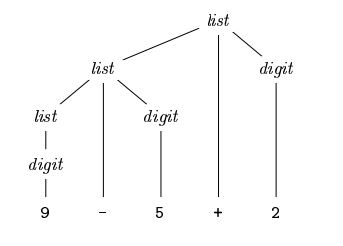
\includegraphics[scale=1]{parseTree.jpg}\end{center}
		\caption{Parse Tree for $G$}
  		\label{fig:parsetree1}
	\end{figure}


\section{Syntax-Directed Definition}
	\subsection{Attributes}
		An attribute is any quantity associated with a programming construct (or grammar symbols (nonterminals and terminals) used to represent programming constructs). Examples of attributes are data types of expressions, the number of instructions in the generated code, or the location of the first instruction in the generated code for a construct, among many other possibilities.
	\subsection{Syntax-Directed Translation Schemes}
		A translation scheme is a notation for attaching program fragments to the productions of a grammar. The program fragments are executed when the production is used during syntax analysis. The combined result of all these fragment executions, in the order induced by the syntax analysis, produces the translation of the program to which this analysis/synthesis process is applied.

	\subsection{Syntax Directed Definition}
		A syntax-directed definition associates
		\begin{itemize}
			\item With each grammar symbol, a set of attributes, and
			\item With each production, a set of semantic rules for computing the values of the attributes associated with the symbols appearing in the production.
		\end{itemize}
		\newpage
		$e.g.$

		\begin{table}[h!]
		  	\begin{tabular}{|l|l|}

		  		\hline
		  		$PRODUCTION$ & $SEMANTIC RULES$\\

		  		\hline \hline

		    	$expr \rightarrow expr_{1} + term$ & $expr.t = expr_{1}.t || term.t || '+'$\\
		    	$expr \rightarrow expr_{1} - term$ & $expr.t = expr_{1}.t || term.t || '-'$\\
		    	$expr \rightarrow term$ & $expr.t = term.t$\\
				$term \rightarrow  0$ & $term.t = '0'$\\
				$term \rightarrow  1$ & $term.t = '0'$\\
				$...$ & $...$ \\
				$term \rightarrow  9$ & $term.t = '9'$\\
				\hline

		  	\end{tabular}
		  	\centering
		  	\caption{Syntax-directed definition for infix to postfix translation}
		  	\label{tab:table1}
		\end{table}

		Table \ref{tab:table1} shows a syntax-directed definition for infix to postfix translation. The attributes are evaluated either while parsing itself, or can be evaluated once the parse tree has been obtained by post-order traversal as illustrated below.

		\begin{algorithm}[h!]
			\caption{Depth First Traversal of Tree}
			\label{alg:alg1}
			\begin{algorithmic}

			\Function{visit}{node $N$}
				\For{each child $C$ of $N$, from left to right}
					\State \Call{visit}{$C$};
					\State evaluate semantic rules at node $N$;
				\EndFor
			\EndFunction
			\end{algorithmic}
		\end{algorithm}


		\begin{figure}[h!]
			\begin{center}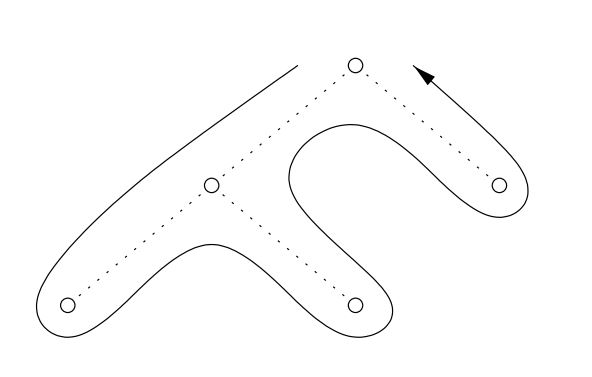
\includegraphics[scale=0.7]{postorder.jpg}\end{center}
			\caption{Example of a depth-First traversal of a tree}
	  		\label{fig:postorder2}
		\end{figure}

	\newpage

		\begin{figure}[h!]
			\begin{center}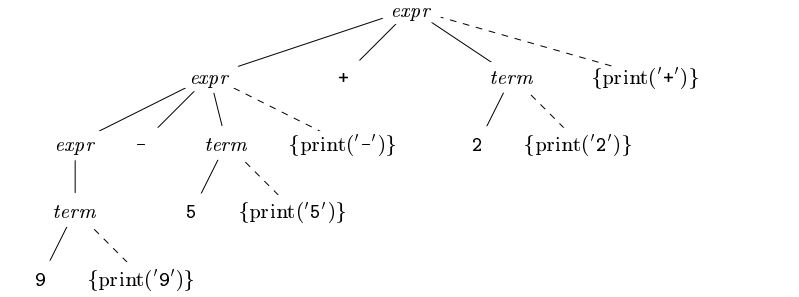
\includegraphics[scale=0.8]{eval.jpg}\end{center}
			\caption{Actions translating $9-5+2$ into $95-2+$}
	  		\label{fig:eval3}
		\end{figure}

\section{Intermediate Code Generation}
	Once a parse tree has been generated, it is passed to a \emph{Semantic Analyzer} which annotates the parse tree (evaluates it's attributes). For \emph{synthesized} attributes, the values are evaluated in a bottom-up order, while \emph{inherited attributes} attributes are evaluated in a top-down order.

	\begin{figure}[h!]
		\begin{center}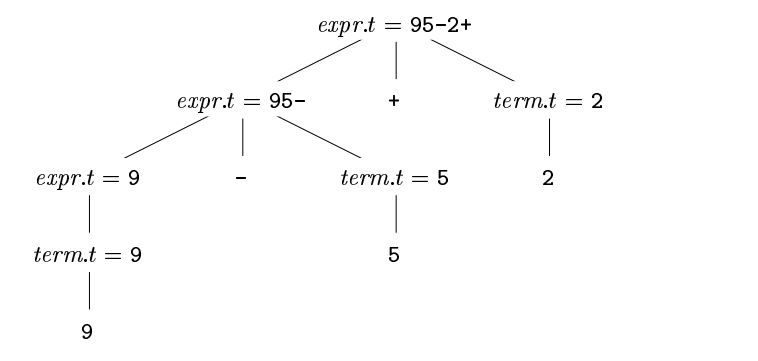
\includegraphics[scale=0.8]{sdd.jpg}\end{center}
		\caption{Attribute values at nodes in a parse tree for SDD in table \ref{tab:table1}}
  		\label{fig:sdd4}
	\end{figure}

	There are many ways of generating intermediate code, one of which is constructing a(n) \emph{(Absract) Syntax Tree}.

\section{Abstract Syntax Tree (AST)}
	An abstract syntax tree (AST), or just \emph{syntax tree}, is a tree representation of the abstract syntactic structure of source code written in a programming language. Each node of the tree denotes a construct occurring in the source code. The syntax is abstract in not representing every detail appearing in the real syntax. While a Parse Tree explicitly shows how the string is derived, the Syntax Tree does away with language-specific details and retains only information relevant to further generation of code in the Target Language. The tree can be constructed by evaluating nodes/labels as attributes of the grammar symbols during parsing (using an SDD) or from the parse tree by post order traversal as shown above. Here we see an example SDD (grammar $H$ and ruleset $R$) that define the language (set) of legal expression strings and describe a procedure to find the nodes (treated here as attributes) of the corresponding AST.

	The SDD for grammar $H$:

	\begin{table}[h!]
	  	\begin{tabular}{|l|l|}

	  		\hline
	  		$PRODUCTION\ of\ H$ & $SEMANTIC RULES (R)$\\

	  		\hline \hline

	    	$E \rightarrow E_{1} + T$ & $E.node = \mathbf{new} \mathit{NODE}(E_{1}.node, T.node, '+')$\\
	    	$E \rightarrow E_{1} - T$ & $E.node = \mathbf{new} \mathit{NODE}(E_{1}.node, T.node, '-')$\\
	    	$E \rightarrow T$ & $E.node = T.node$\\
			$T \rightarrow (E)$ & $T.node = E.node$\\
			$T \rightarrow \mathbf{id}$ & $T.node = \mathbf{new} \mathit{LEAF}(\mathbf{id}, \mathbf{id}.\mathit{entry}$\\
			$T \rightarrow \mathbf{num}$ & $T.node = \mathbf{new} \mathit{LEAF}(\mathbf{num}, \mathbf{num}.\mathit{entry}$\\
			\hline

	  	\end{tabular}
	  	\centering
	  	\caption{Constructing syntax trees for simple expressions using and SDD}
	  	\label{tab:table2}
	\end{table}


	\begin{figure}[h!]
		\begin{center}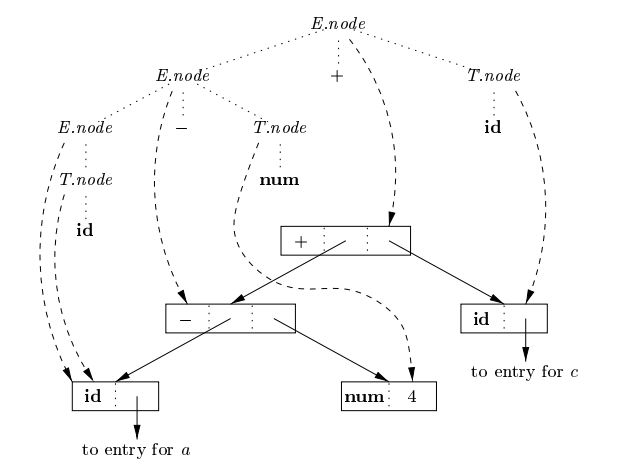
\includegraphics[scale=0.8]{stree.jpg}\end{center}
		\caption{Syntax tree for $a - 4 + c$ using SDD in Table \ref{tab:table2}}
  		\label{fig:stree5}
	\end{figure}

\section{References}

	All examples and illustrations were sourced from:
	Aho, Alfred V.; Lam, Monica S.; Sethi, Ravi; Ullman, Jeffrey D. \textbf{\emph{Compilers, Principles, Techniques, and Tools (Second edition).}}

\section{Gate Questions}

	\subsection{Gate}
		In the context of abstract-syntax-tree (AST) and control-flow-graph (CFG), which one of the following is True?
		\renewcommand{\labelenumi}{\Alph{enumi}}
		\begin{enumerate}\bfseries
			\item In both AST and CFG, let node N2 be the successor of node N1. In the input program, the code corresponding to N2 is present after the code corresponding to N1
			\item For any input program, neither AST nor CFG will contain a cycle
			\item The maximum number of successors of a node in an AST and a CFG depends on the input program
			\item Each node in AST and CFG corresponds to at most one statement in the input program
		\end{enumerate}

		\newpage

		The answer is \textbf{(C)}, as:\\\\
		A control flow graph (CFG) is a representation, using graph notation, of all paths that might be traversed through a program during its execution. Each node corresponds to a block of code, and each edge corresponds to the transfer of control between blocks of code.
		

		\begin{enumerate}
		\item is false, In a CFG (Control Flow Graph), the code of N2
		may be present before N1 when there is a loop or goto.

		\item is false, a CFG (Control Flow Graph) contains cycle
		when input program has loop.

		\item is true, successors of ASTs and CFGs depend on
		input program

		\item is false, a single node may correspond to a block
		of statements.
		\end{enumerate}


\end{document}